\documentclass[a5paper, 12pt, twoside]{article}

% \usepackage[a5paper,left=2cm,right=1cm,top=1cm, bottom=1.5cm]{geometry}
\usepackage{array}
\usepackage{makecell}
\usepackage{ulem}
\usepackage[all]{nowidow}
\usepackage{wrapfig}
\usepackage{enumitem}
\usepackage{multicol}

% \usepackage{hyperref}
% \hypersetup{
%     colorlinks=true,
%     urlcolor=sokolblue,
%     }

\usepackage[czech]{babel}
\usepackage[utf8]{inputenc} 
\usepackage{ellipsis}

\usepackage{fontspec}
\newfontfamily{\tyrs}{Sokol Tyrs}
\newfontfamily{\fugner}{Sokol Fugner}

% \usepackage{lmodern}
% \usepackage[T1]{fontenc} 

\usepackage{anyfontsize}
\newcommand{\titlesize}{\fontsize{56pt}{67pt}}


\usepackage[dvipsnames]{xcolor}
\definecolor{sokolred}{RGB}{228, 5, 33}
\definecolor{sokoldarkred}{RGB}{200, 0, 30}
\definecolor{sokolblue}{RGB}{45, 46, 135}

\usepackage{tikz}
\usetikzlibrary{calc}

\newcommand{\pozned}[1]{%
\textit{#1}}

% \newcommand{\post}[1]{%
% \begin{center}
% {\huge \tyrs #1}
% \end{center}
% }

% \newcommand{\subpost}[1]{%
% \vspace*{12pt}
% \begin{center}
% {\Large \tyrs #1}
% \end{center}}

% \newcommand{\signature}[2]{%
%   \begin{flushright}
%     \textbf{#1}\\#2
%   \end{flushright}
% }

% \newcommand{\luv}{\clqq\kern-0.07em}
% \newcommand{\ruv}{\kern0.07em\crqq\kern0.1em}


\usepackage{csquotes}
\DeclareQuoteAlias{german}{czech}
\MakeOuterQuote{"}

\usepackage{ebgaramond}

\setlength{\voffset}{-30mm}
% \setlength{\hoffset}{-25mm}
\setlength{\textheight}{170mm}
\setlength{\textwidth}{116mm} %120
\setlength{\oddsidemargin}{-4mm}
\setlength{\evensidemargin}{-14mm} %13 15

\setlength{\parskip}{0pt}

% \addtolength{\oddsidemargin}{-4mm} \addtolength{\evensidemargin}{-4mm} %% printer shift

% \usepackage[1to1]{booklet}
% \pagespersignature{16}
% \target{\magstep0}{297mm}{210mm}

% \ifpdf % from the ifpdf package
% 	\pdfoutput = 1 % generate pdf output
% 	\setpdftargetpages % set output page size
% \else
% 	\setdvipstargetpages % use this for dvi output
% \fi

% \addto\captionsczech{\renewcommand{\chaptername}{}}
% \addto\captionsczech{\renewcommand{\thechapter}{}}
\addto\captionsczech{\renewcommand{\contentsname}{Obsah}}

% \addtopsmarks{headings}{}{
%   \createmark{chapter}{left}{shownumber}{}{}
% }
% \pagestyle{headings}


\setcounter{secnumdepth}{0}

\usepackage[textfont=it]{caption}
\usepackage[textfont=it]{subcaption}

\begin{document}

%% obálka
\pagecolor{sokolred}
\color{white}
\pagenumbering{gobble}
\begin{center}

  \vspace*{\fill}

  \includegraphics*[width=0.9\textwidth]{./Sokolovna-kresba-white.png}

  \vspace{134pt}

  {\titlesize\fugner Almanach}

  {\titlesize\tyrs SOKOLA LIBEŇ}

  \vspace*{\fill}
\end{center}
\clearpage

\normalcolor
\nopagecolor

\null\clearpage

% titulka
\begin{center}

  \vspace*{\fill}

  \includegraphics*[width=0.9\textwidth]{./Sokolovna-kresba-black.png}

  \vspace{134pt}

  {\titlesize\fugner Almanach}

  {\titlesize\tyrs SOKOLA LIBEŇ}


  \vspace*{\fill}
\end{center}

\mbox{}
\clearpage

% ISBN
\vspace*{\fill}
{ \parindent0pt \parskip6pt
140 let tělocvičné jednoty Sokol Praha-Libeň

Editor: Jan Přech 

Grafická úprava: Martin Burian 

Jazyková úprava: Martina Waclawičová

1. vydání 

Vyšlo v~Praze nákladem T.~J. Sokol Libeň při příležitosti 140. výročí založení jednoty v~roce 2024.

© 2024 T.~J. Sokol Praha-Libeň

ISBN 978-80-11-05742-8
}
\clearpage

% Obsah

\tableofcontents

\clearpage

% \mainmatter

\pagenumbering{arabic}

\section{Úvod}

Sestry a bratři, dámy a pánové, ctění čtenáři,

\noindent již 140 let je tělocvičná jednota Sokol v~Libni místním hybatelem sportovního i společenského života. V~duchu myšlenek dr. Miroslava Tyrše a Jindřicha Fügnera, zakladatelů Sokola, se snažíme přibližovat naše členy antickému ideálu kalokagathie, tedy dokonalosti ducha i těla. Sokol je vnímán především jako sportovní organizace, přinášel a přináší sport pro každého, bez rozdílu věku a příjmu. Rozvíjí tělesnou zdatnost svých členů i ostatních. Ale Sokol je a byl také vlastenecký v~nejlepším slova smyslu. Své členy vede k~lásce k~rodné zemi a k~úctě k~duchovnímu dědictví našeho národa. Sehrál klíčovou roli při vzniku československých legií a ustavení naší novodobé státnosti. Stejně tak vždy byl a dnes je i hybatelem kulturních aktivit. V~neposlední řadě spojoval a spojuje členky a členy rozdílných společenských postavení, profesí, politických přesvědčení a životních zkušeností při společné aktivitě. Jsem přesvědčen, že to je klíčová úloha Sokola v~dnešních dnech, kdy mnozí společnost aktivně rozdělují a straší pro své partikulární zájmy, než aby ji spojovali a postavili se skutečným výzvám naší doby. 

U~příležitosti 140. výročí naší jednoty jsme se rozhodli vydat doplněný almanach mapující historii jednoty od jejího založení do současnosti. Almanach téměř beze změn přejímá texty z~vydání u~příležitosti 120. výročí založení jednoty (2004) a doplňuje je o~shrnutí posledních 20 let s~ambicí být i historickým pramenem pro budoucnost. 

Jelikož almanach je souborem příspěvků různých pamětníků, některé události jsou zmíněny na více místech, vždy v~kontextu daného příspěvku a nikoliv přísně chronologicky. Jsem nicméně přesvědčen, že tato vyprávěcí forma bude pro čtenáře příjemnější než encyklopedická. 

\vspace{\baselineskip}
\hfill\textit{Jan Přech}

\hfill\textit{jednatel T.~J. Sokol Libeň}

\hfill\textit{editor almanachu ke 140 letům jednoty}

\section{Úvodní slovo starosty br. Jiřího Sixty ke 120.~výročí založení jednoty}

V~roce 2004 si připomínáme 120. výročí založení Tělocvičné jednoty "Sokol" v~Praze-Libni, která byla obnovena po době, kdy nebylo možné se veřejně hlásit k~sokolským ideálům.

Ku příležitosti tohoto významného výročí jsme se rozhodli nejen uspořádat slavnostní Akademii a výstavu, ale vydat také Almanach, který bude mapovat vývoj činnosti v~naší jednotě od založení až po současnost. Výsledek našeho snažení držíte právě v~rukou.

Velkou zásluhu na znovuobnovení sokolské činnosti v~roce 1990 mají kromě jiných, pamětníci slavné sokolské éry, kteří svými zkušenostmi v~sokolském hnutí a s~obětavým osobním nasazením, započali novou etapu sokolských aktivit v~Libni až do současnosti. Také díky nim byla naše jednota opět zaregistrována 16. července 1990 pod názvem Tělocvičná jednota Sokol Libeň. V~roce 1991 se rozbíhají v~navrácené sokolovně aktivity v~sokolské všestrannosti, sportovních a turistických oddílech a společenských akcích vzdělavatelského sboru. Rychle se rozrůstá členská základna. Velké množství cvičenců a dobrovolných pořadatelů z~libeňské jednoty se podílelo na zdárném průběhu XII. všesokolského sletu 1994 a XIII. všesokolského sletu 2000. Již brzy se rozběhnou přípravy na XIV. všesokolský slet v~roce 2006, do kterého se i naše jednota hodlá aktivně zapojit.

Budovu sokolovny, která se nacházela v~době převzetí ve špatném technickém stavu, bylo nutné začít postupně v~závislosti na finančních prostředcích uvádět do provozuschopného stavu. Po rekonstrukci fasády a střechy v~roce 2002 se libeňská sokolovna opět stala jednou z~dominant centrální části Libně. Dokončení rekonstrukce sokolovny, která byla v~roce 2001 prohlášena za kulturní památku, bude stát ještě nemálo úsilí a finančních prostředků.

V~současné době je naším prvořadým úkolem práce s~nastupující mladou generací. I~v~dnešní uspěchané době je třeba dbát o~její všestranný tělesný i duševní rozvoj. Díky obětavosti mnoha cvičitelů a činovníků bude proto náš libeňský Sokol i nadále vzkvétat.

Přeji naší jednotě k~jejímu 120. výročí mnoho zdaru a úspěchu do dalších let, obětavé cvičitele a činovníky a mnoho spokojených členů.

\clearpage

\section{Založení T.~J. Sokol Libeň}
\subsection{První kroky}
Historii jednoty až do roku 1984 sepsal: br. Adolf Peťule (1908–1987)

\begin{center}
  \textit{"V pravdě stůj, vlast miluj, nechtěj porobu, služ vlasti, národu!"}
\end{center}

\noindent Slova chorálu v~závěru vystoupení mužského dorostu na VIII. sletu všesokolském v~roce 1926 byla již o~42 let dříve vůdčím heslem několika pokrokových a vlasteneckých občanů, jež osud zavál do tehdejší vesnice Libně, v~okresu karlínském, aby tu byli šiřiteli národní osvěty. Buďte zde pro trvalou a oživovanou paměť zachována jejich jména:

\textbf{Ladislav Verner}, nar. 7. 1. 1856 v~Byháni, učitel obecné školy chlapecké od 21. 4. 1882.

\textbf{Jaroslav Pechan}, nar. 15. 10. 1862 v~Praze, od 2. 11. 1882 zatímní podučitel do 5. 8. 1886, kdy odešel do Kozel.

\textbf{František Gliman}, nar. 6. 5. 1862 v~Chocni, dočasný smluvní učitel od 1. 9. 1882, odešel do Nehvizd 1. 3. 1886.

\textbf{Václav Kalaš}, provizorní podučitel od 2. 11. 1882, odešel do Prahy 9. 12. 1885.

Tito čtyři mladí učitelští mládenci (z~nichž Jaroslav Pechan již od roku 1880 je členem-stipendistou Sokola Pražského a tedy pod přímým vlivem Dr. Miroslava Tyrše i jako cvičitel jeho Tělocvičného ústavu pro hochy), našli ubytování ve třech místnostech v~tzv. staré faře Dr. Košáka.

\begin{figure*}[h]
  \centering
  \begin{subfigure}{0.45\textwidth}
  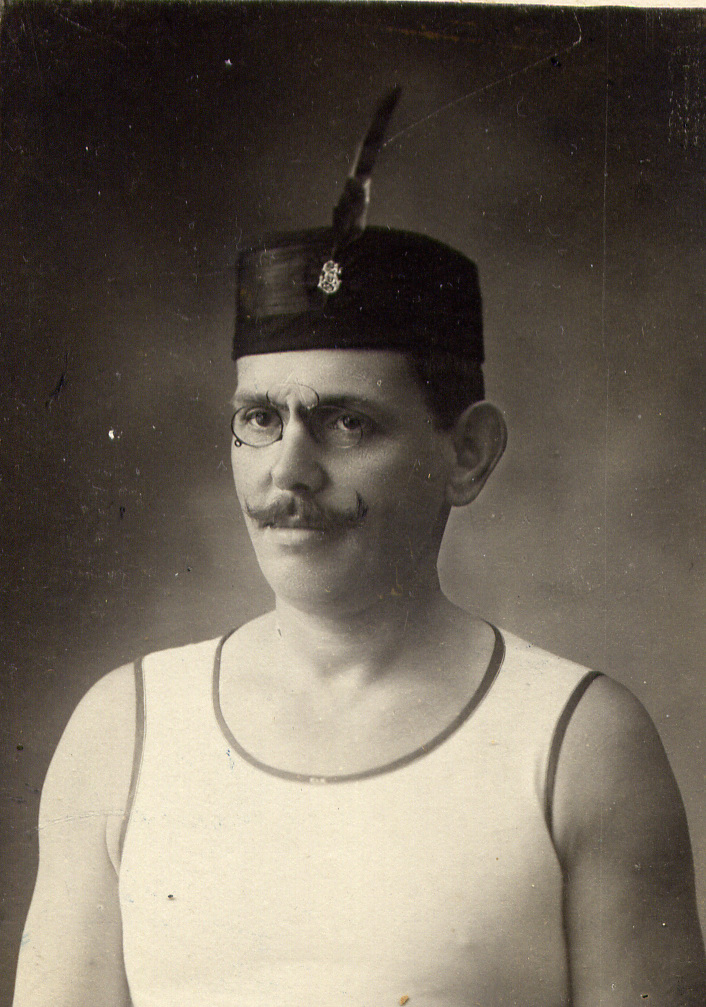
\includegraphics[width=\textwidth]{img/pechan.jpg}
  \caption*{br. Jaroslav Pechan, zakládající člen jednoty, foto: archiv T.~J. Sokol Libeň}
  \end{subfigure}
  \hfill
  \begin{subfigure}{0.45\textwidth}
  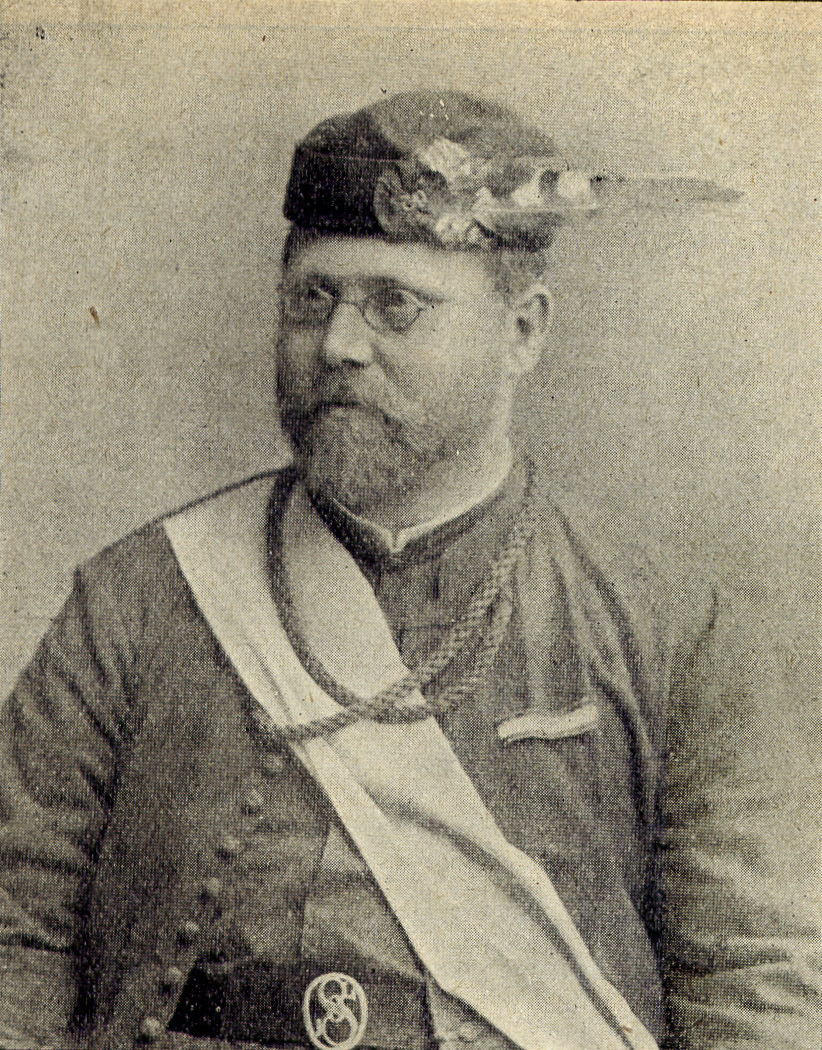
\includegraphics[width=\textwidth]{img/klazar.jpg}
  \caption*{JUC. Václav Klazar, první náčelník T.~J. Sokol Libeň (1884–⁠⁠⁠⁠⁠⁠1890) a druhý starosta (1895–⁠⁠⁠⁠⁠⁠1899), foto: archiv T.~J. Sokol Libeň}
  \end{subfigure}
\end{figure*}

I~u~nás, v~chudém dělnickém prostředí, byla již tehdy německá škola (vliv německých továrních firem) a na dveřích obecního úřadu cedule: "Mluvte česky! Kdo se za svůj jazyk stydí, hoden potupy všech lidí!", kterou tam vyvěsil tajemník obecního úřadu JUC. Václav Klazar, rovněž činný člen Sokola Pražského (od roku 1879). Není tedy divu, že tito mladí idealisté – a mohl mladý učitel na venkovské škole nebýt idealistou? – si uvědomili nejen velký význam a vliv Tyršových myšlenek, ale i svou učitelskou odpovědnost.

Bylo tehdy v~Čechách a na Moravě po l. všesokolském sletu (1882) již 104 sokolských jednot a v~blízkosti Libně sedm: V~Praze (zal. 1862), V~Karlíně (1867), na Smíchově (1868), ve Vršovicích (1870), v~Záběhlicích (1870), v~Braníku (1871) a na Žižkově (1872), nehledě k~sedmi jednotám v~ostatní Evropě a dvaceti v~USA. Snadné se dohodnout – nesnadné provést, zvláště v~takovém malém i společensky nevýhodném prostředí. Ale i tady se cesta našla. Dne 8. září 1884 byla uspořádána v~tehdejším hostinci "U Deutschů" přednáška náměstka náčelníka Sokola Pražského Dr. Františka Čížka o~úkolech a cílech sokolského hnutí. Zúčastnilo se jí kupodivu 118 osob. Řídil ji Tomáš Ronek.

\begin{figure*}[h]
  \centering
  \begin{subfigure}[c]{0.4\textwidth}
  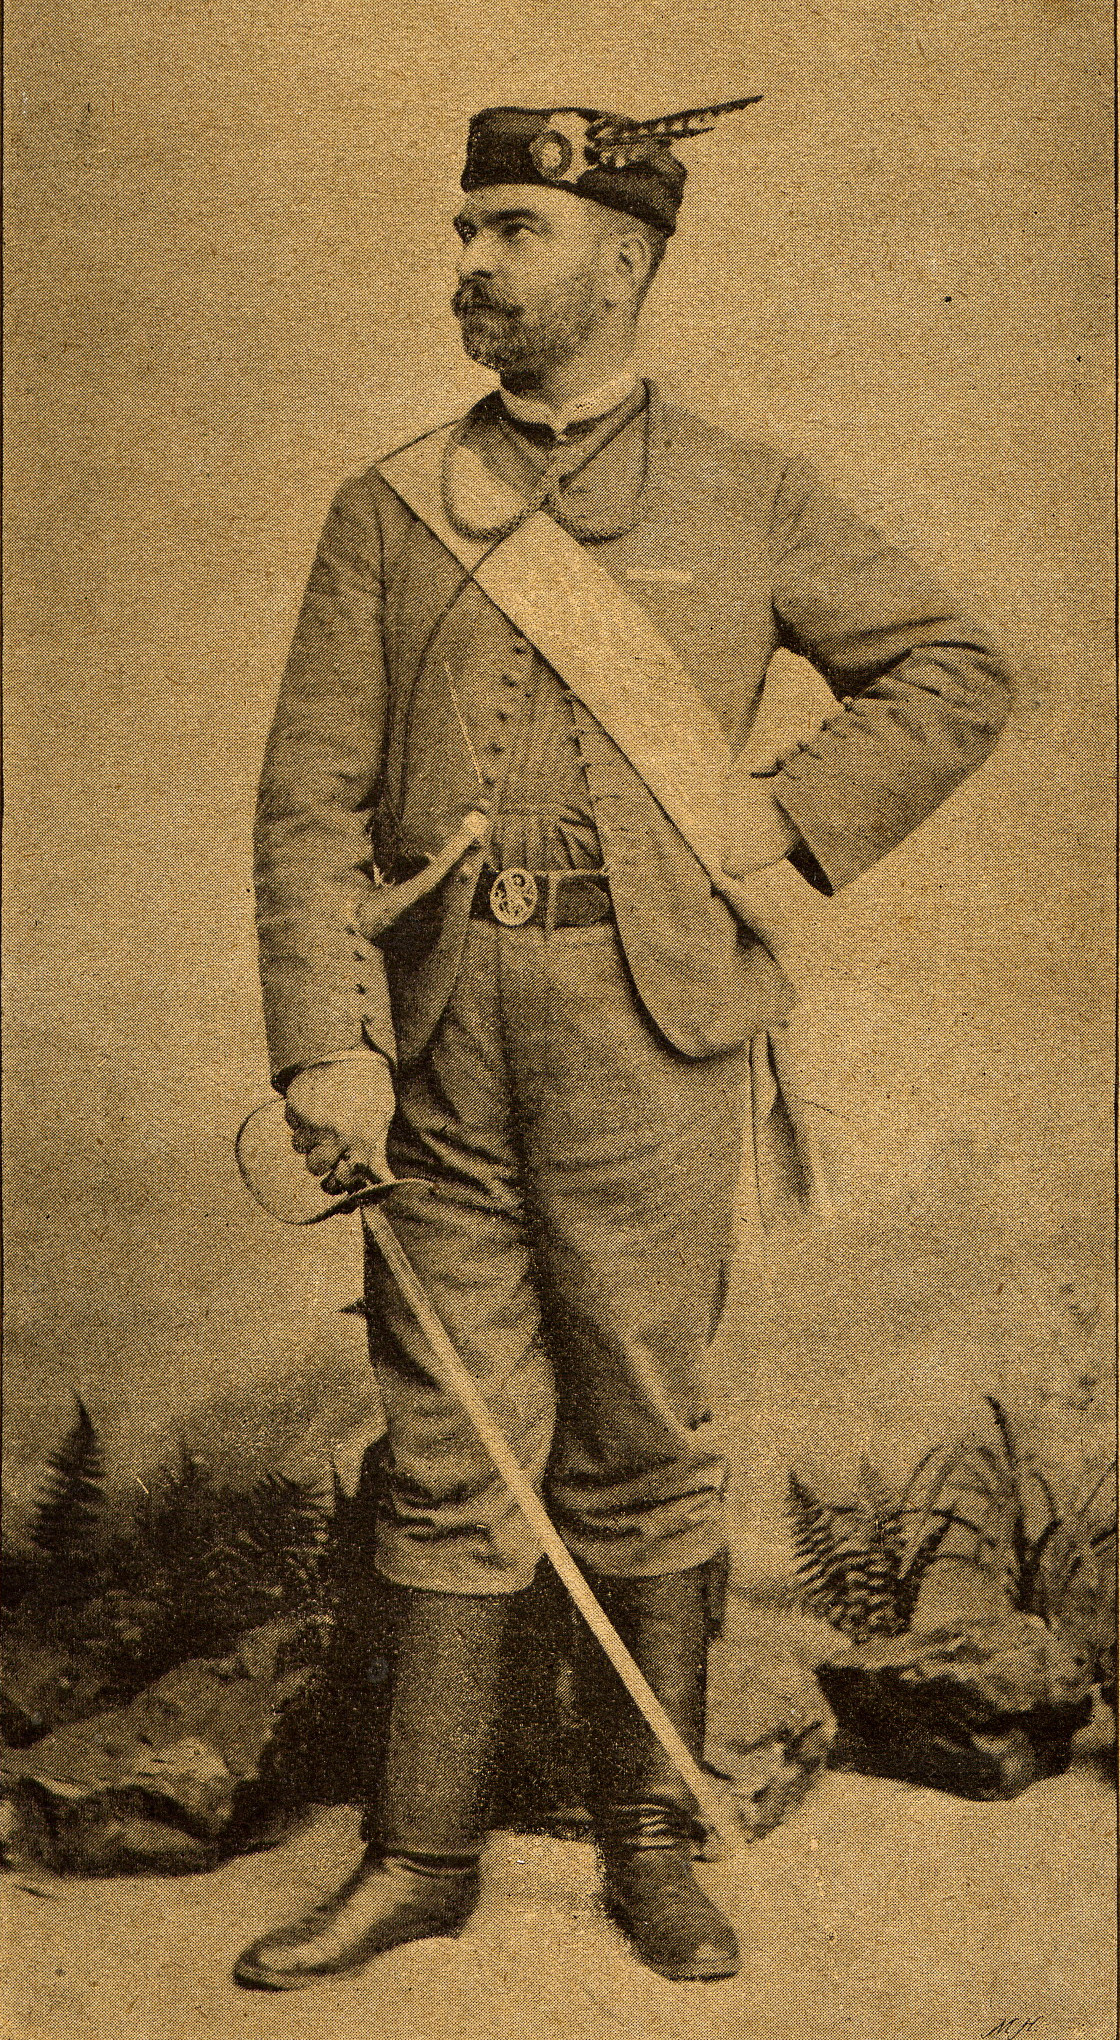
\includegraphics[width=\textwidth]{img/cizek.jpg}
  \caption*{Dr. František Čížek, zakládající člen jednoty (1884), foto: archiv T.~J. Sokol Libeň }
  \end{subfigure}
  \hfill
  \begin{subfigure}[c]{0.5\textwidth}
  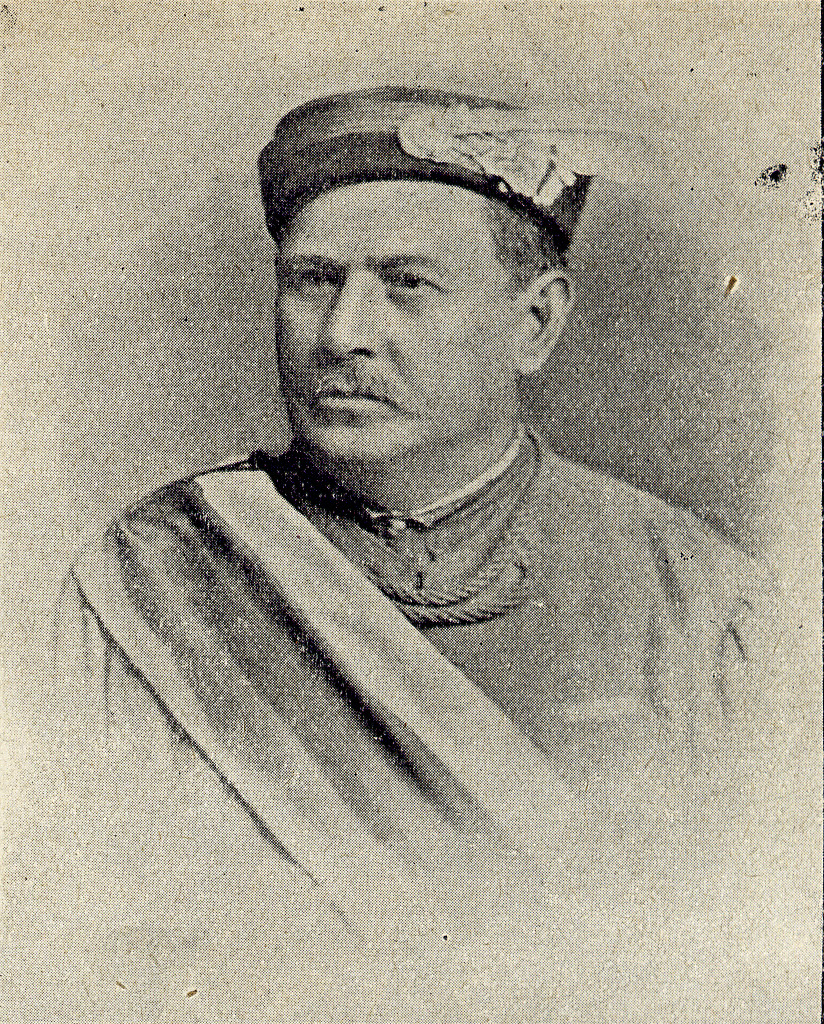
\includegraphics[width=\textwidth]{img/voctar.jpg}
  \caption*{Josef Voctář, první starosta T.~J. Sokol Libeň (1884–⁠⁠⁠⁠⁠⁠1894), foto: archiv T.~J. Sokol Libeň }
  \end{subfigure}
\end{figure*}

K~vlastnímu založení T.~J. Sokol v~Libni došlo pak v~ustavující valné hromadě 26. 10. 1884, při níž byl za starostu obezřetně zvolen obecní starosta Josef Voctář, jeho náměstkem "stavitel ve službách obecních" Josef Bukovský, náčelníkem JUC. Václav Klazar, jeho náměstkem učitel Jaroslav Pechan a jednatelem Vítězslav Vondřich. Bylo tedy vedení jednoty svěřeno osobám odborně povolaným, ale i důvěryhodným, neboť ne všemu obyvatelstvu mohlo být vítáno pokrokové zaměření Sokola, bratrské tykání, pozdrav "Nazdar" a dokonce červená košile sokolského kroje.

Cvičit se počalo velmi brzy; již 20. ledna 1885. Cvičilo se první tři léta v~hostinci u~Deutschů, později se souhlasem místní školní rady ve škole a pro letní cvičení byl získán roku 1887 od obce pozemek ve výměře 200 čtverečních sáhů po 10 haléřích, jenž byl později vyměněn za jiný, o~40 sáhů větší (1 čtvereční sáh = 3,6\,$\textrm{m}^2$).

Duší tělocvičné činnosti byl od počátku bratr Jaroslav Pechan, později středoškolský profesor tělocviku, horlivý propagátor tělesné výchovy školní i sokolské. Podlehl posléze dlouholeté chorobě, jež přerušovala jeho nadějnou činnost. Byl autorem "Osnov k~vyučování tělocviku na školách středních, díl I." (r. 1905) a "Tělocviku pro obecné školy chlapecké na základě soustavy Miroslava Tyrše, díl I." (r. 1888). O~Pechanových vlastnostech a zásluhách můžeme číst v~"Památníku 25 letého trvání T.~J.  Sokol v~Praze-Libni 1884–⁠⁠⁠⁠⁠⁠1909" z~pera Františka Glimana a Památníku z~roku 1934 z~pera Ladislava Vernera, dvou jeho současníků a spolupracovníků. Pozdější místonáčelník jednoty, všestranný umělec, český básník, autor "Sokolských sonetů" a odborný sokolský tělocvičný spisovatel Karel Hlaváček (1874-1898) o~něm napsal: "Na prvním místě bije do očí jeho neúnavná činnost, která vrcholí ve dnech župního sletu roku 1886, kdy bydlil dávno již na místě vzdáleném a přece svou pevnou rukou ovládal a řídil přípravné kroky. Byl vychovatelem sokolských  charakterů.  Chválím si bratra Pechana jako bystrovtipného organizátora, jenž řady všech odborů upevnil tuhou kázní řádů zocelil a utužil. Bude vždy mezi předními, jež slaviti a vzpomínati budeme jako muže o~jednotu zasloužilé." Roku 1889 tento v~tělocviku odborně kovaný J. Pechan je již náčelníkem Sokola Vinohradského. Jeho duch v~cvičitelském sboru opravdu na dlouho přetrval jeho odchod. Zemřel 14. 6 .1915 v~Praze a pohřben byl na Vinohradském hřbitově.

\begin{figure*}[h!]
  \centering
  \includegraphics[width=0.9\textwidth]{img/zakladajici_clenove_1886.jpg}
  \caption*{Členové jednoty v~roce 1886, uprostřed s~plnovousem JUC. Václav Klazar, t.č. náčelník a ve druhé řadě druhý z~prava starosta Josef Voctář; foto: archiv T.~J. Sokol Libeň}
\end{figure*}

Vedle pravidelného cvičení od počátku byl pěstován i život společenský. Téměř pravidelně byly pořádány tradiční sokolské "Šibřinky" u~Deutschů, nebo v~pivovarnickém sále (v~některých letech nahrazeny subskripcí rozmnožující finanční prostředky jednoty), čajové večírky, z~nichž jeden navštívil sám Mikoláš Aleš. Pěstovány byly též přátelské styky s~jinými jednotami (společný výlet do Kunratic se Sokolem Pražským r. 1886). Členové se navštěvovali v~jednotách, účastnili se pohřbů známých a zasloužilých osob (např. Dr. Ed. Grégra, přenesení ostatků P. J. Šafaříka, Jana Kollára apod.). Do pravidelné činnosti jednoty patřily každý rok četné výlety, krátké, delší, denní i noční. Bývaly spojeny příznačně pro tu dobu s~různými slavnostmi, veřejným cvičením a pod., jako akce národně vlastenecké a společenské zároveň utužující vzájemnou, tehdy tak potřebnou, pospolitost vskutku bratrského ducha a posilující i tělesně. Účastnil se jich také někdy trubačský sbor jednoty založený již roku 1886. Tento trubačský sbor sdílel za sbormistrů Arona, Šerkse a Šillera téměř deset let osudy jednoty na nestálé a kolísavé vlně práce, úspěchů a přízně i horlivosti členů. Již roku 1887 si stěžuje kronikář, že vojenské odvody jeho řady prosívají na čtvrtinu. Nakonec se sbor v~roce 1895 rozešel. Roku 1904 byl sice na čas vzkříšen, ale skutečné obnovy se dočkal až v~roce 1910.

\begin{figure*}[h!]
  \centering
  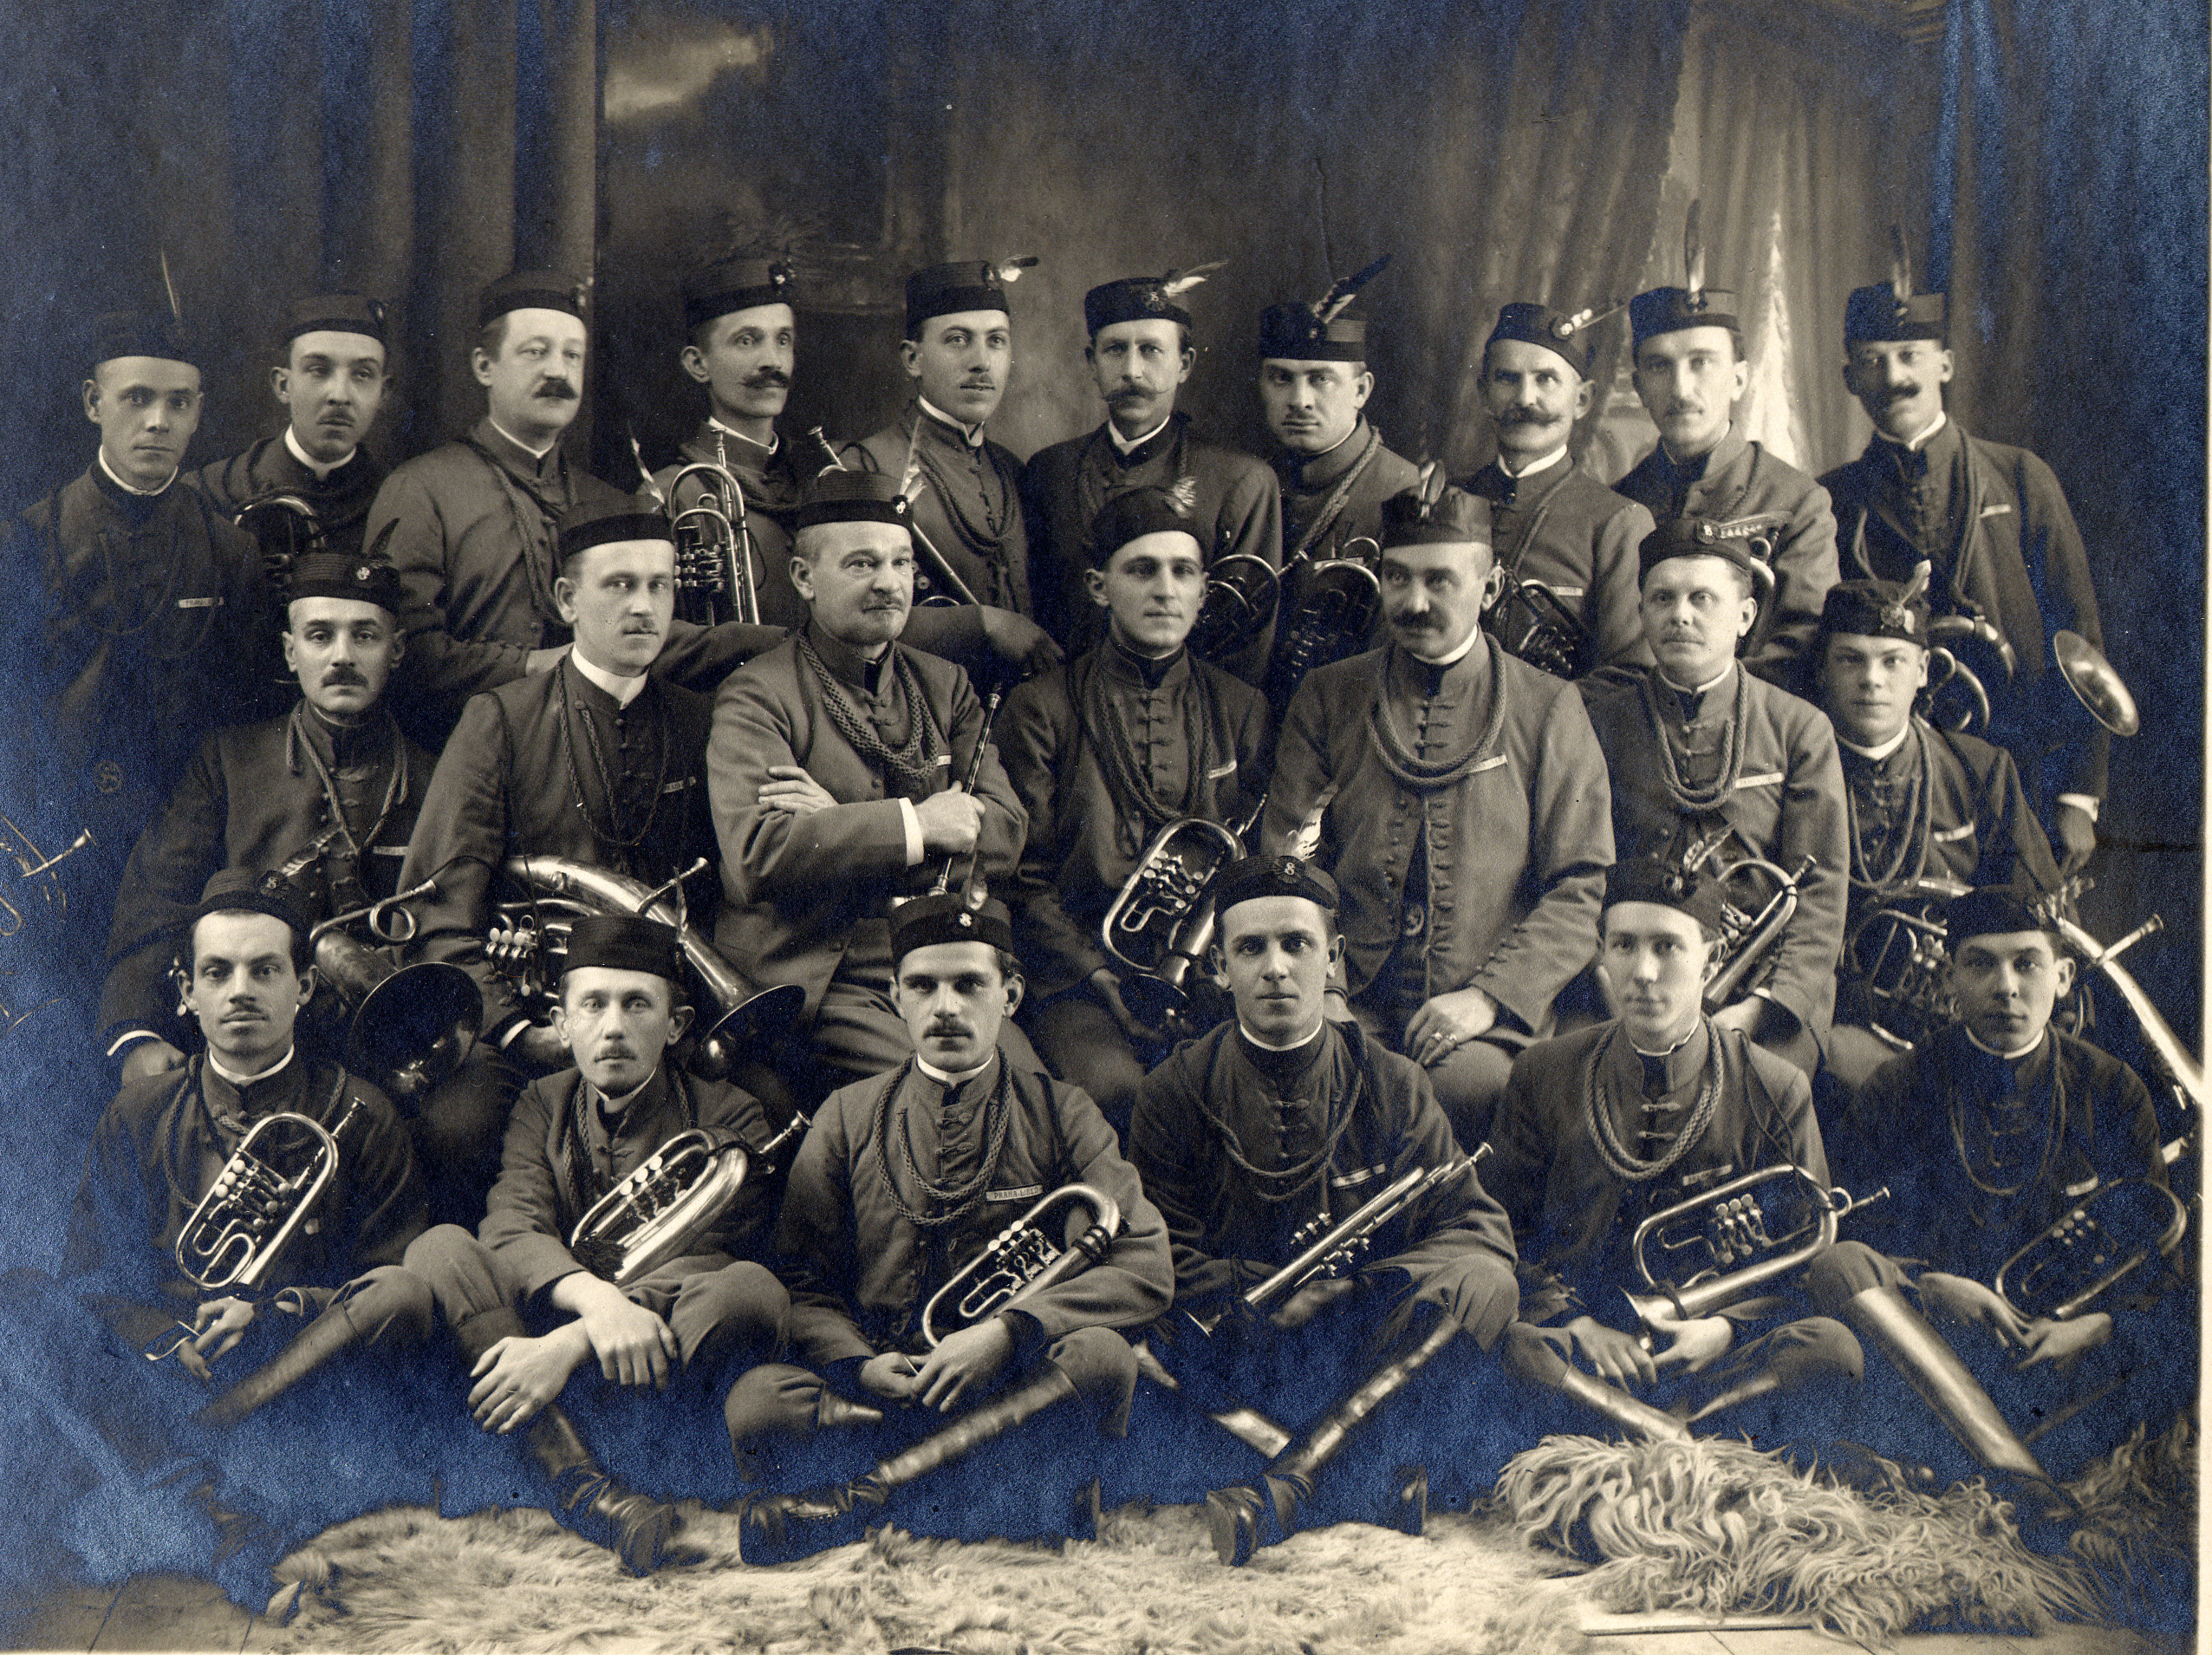
\includegraphics[width=0.9\textwidth]{img/trubaci.jpg}
  \caption*{Trubačský sbor jednoty (1886), foto: archiv T.~J. Sokol Libeň}
\end{figure*}

Časté byly též zájezdy do jiných měst a jednot při nejrozmanitějších příležitostech (např. 1893 zájezd do Polska, 1898 Palackého oslavy v~Hodslavicích, 1900 zájezd ČOS do Olomouce, 1903 slet v~Českých Budějovicích, 1905 Vídeň, 1906 Záhřeb aj.). V~posledních letech tohoto období došlo k~úspěšnému pravidelnému pořádání členských besed s~hodnotnou náplní a hojných vycházek v~našem hlavním městě s~návštěvami památek a uměleckých výstav.

Již od vzniku jednoty byly pěstovány přátelské styky také s~rozličnými libeňskými spolky a organizacemi: spolkem "Osvěta-Omladina", s~"Věnceslavem", který vystupoval často i na podnicích jednoty i při zájezdech, "Ústřední maticí školskou" aj. Byla to vůbec doba všestranné nadšené veřejné práce, jež dovedla r. 1889 tři sokolská závodní družstva s~JUDr. Janem Podlipným, přes výslovný osobní zákaz samého c. k. místodržitele, do Paříže pro první tři ceny v~mezinárodních závodech družstev v~tělocviku. V~prvním družstvu byl také spoluzakladatel libeňského Sokola Jaroslav Pechan.

Cvičilo se, někdy s~obtížemi, u~Deutschů, pak v~libeňských školách, když došlo k~neshodám s~hostinským. Cvičilo se i na prostorách kolem sokolovny (po jejím postavení, dnes zahrádka a garáže; \pozned{dnešní dvůr a zahrada sokolovny, pozn. ed.}), nebo na letním cvičišti za "starou hospodou" (1900). Nebyly vždy radostné chvíle také při úvahách, kde cvičit - ale vždy uspěl lidský rozum a pocit odpovědnosti. 

Po organizační stránce měla jednota v~župní organizaci (župní zřízení zavedeno v~Sokole právě roce 1884) své místo v~župě Středočeské a teprve po ustavení České obce sokolské (1889), jejímž prvním starostou byl právě u~nás v~Libni dobře známý JUDr. Jan Podlipný (starosta města Prahy, první starosta Všeslovanského sokolstva), byla přeřazena do župy Barákovy \pozned{(dnes je naše jednota opět součástí župy středočeské J. Podlipného, pozn. ed.)}. V~jejím vedení se vždy dobře uplatňovala. Cvičitelské kurzy pro cvičitele všech složek jednoty, konané v~rámci župy a jednoty, přispívaly k~potřebné odborné úrovni vší práce v~jednotě.

Roku 1896 upravena v~sokolstvu péče o~jednoty v~menšinách, založen základ (fond) pro stavbu menšinových sokoloven a určeny vznikajícím a malým jednotám ve zněmčeném pohraničí tzv. ochranitelky. Byla to nutná pomoc těžce ale odvážně zakládaným jednotám. Sokolské jednotě v~Libni také přidělena "chráněnka" – jednota v~hornických Kopistech u~Mostu, kde snad nebylo ani 200 domů a necelých 2000 obyvatel, jen z~poloviny Čechů. Osada ta patřila mezi nejstarší a nejdůležitější v~celém kraji. Zanikla roku 1979, kdy musela ustoupit uhelným dolům. Jednotu v~Kopistech libeňští pravidelně podporovali, každého jejího podniku se zúčastnili a v~letech 1899 a 1904 k~ní uspořádali hromadné výlety. Roku 1906, kdy se v~Kopistech konal slet župy Krušnohorské, se z~Libně zúčastnilo 35 mužů a 6 žen, v~čele se starostou F. Filipem.

\begin{figure*}[h!]
  \centering
  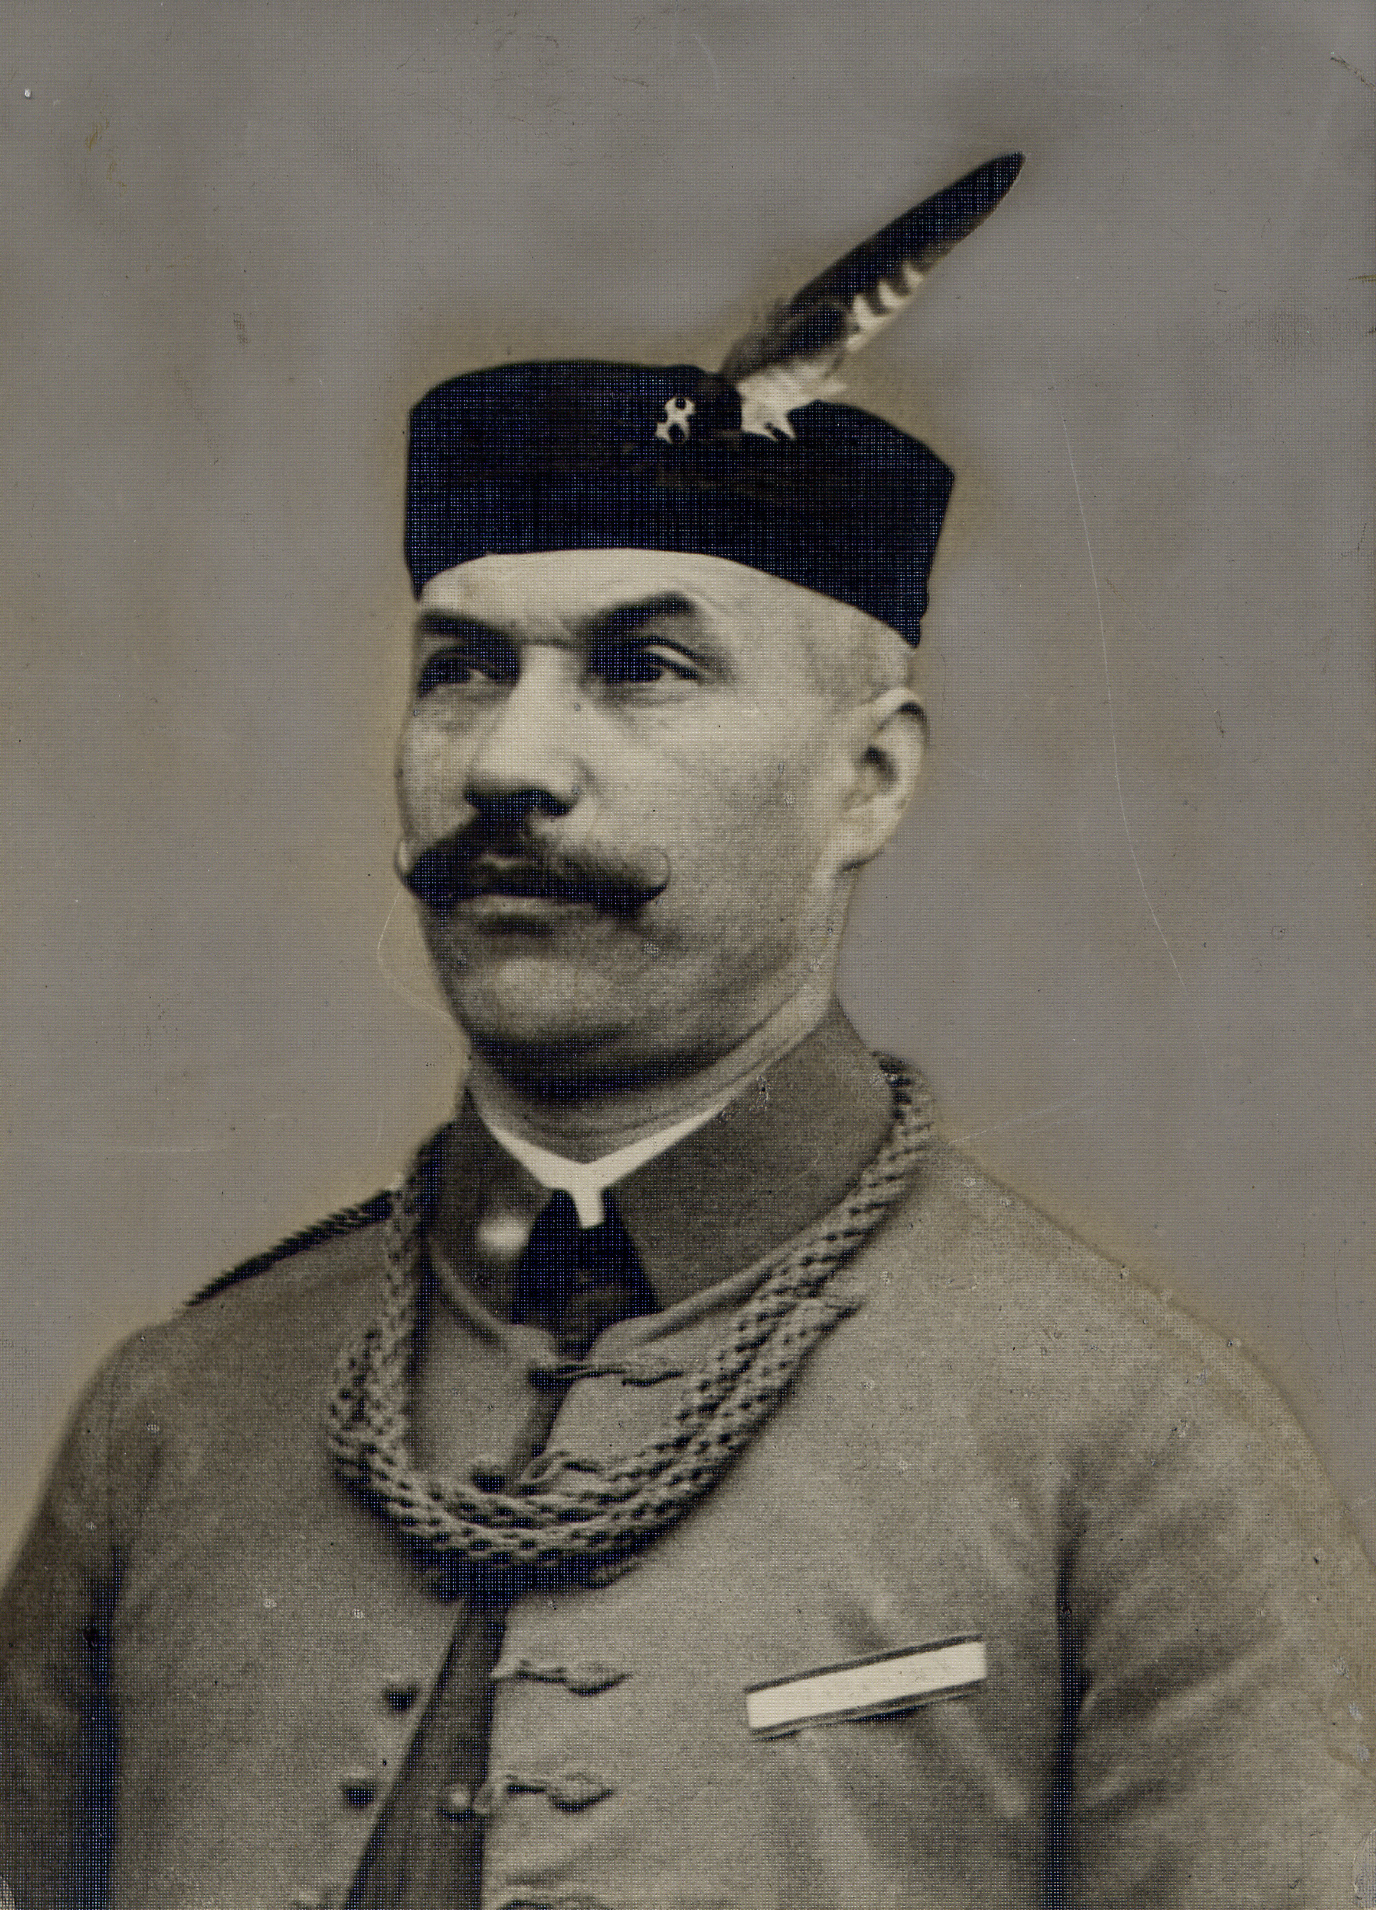
\includegraphics[width=0.4\textwidth]{img/filip_starosta.jpg}
  \caption*{br. František Filip, třetí starosta jednoty (1900–⁠⁠⁠⁠⁠⁠1920); jeho zásluhou byla postavena sokolovna, foto: archiv T.~J. Sokol Libeň}
\end{figure*}

\subsection{První cvičení u~Deutschů}
Zmínili jsme se již o~I. sletu (1882), který se konal na Střeleckém ostrově za osobního řízení Dr. M. Tyrše. Slet přispěl ke vzniku nových sokolských jednot a tak se zrodil i Sokol v~Libni. Přinášíme obrázek hostince u~Deutschů (stál v~místech nynějšího divadla Pod Palmovkou), kde se konala 26. října 1884 ustavující valná hromada a kde první tři roky mladá sokolská jednota cvičila. Už v~prvních cvičeních zde nastupovala tři desetičlenná družstva – bylo to 20. ledna 1885 a již 31. ledna zde uspořádali první šibřinky. Měly ráz: "Praha a okolní obce za sto let". Kronikář Glimann píše: "Výtěžek Šibřinek byl značný. Tak mělo konečně členstvo svoje nářadí a my řadu členů a příznivců více".

V~roce 1886, tj. dva roky po založení jednoty, se konal v~Libni na Knoblochově louce (Libeň tehdy byla ještě vesnicí) župní slet. Byl velmi zdařilý, protože cvičitelský sbor vedený ještě Jaroslavem Pechanem, pracoval naprosto spolehlivě. Je úžasné, co mladá jednota všechno stihla. Těch výletů, doložených "Výletními listy", těch okrskových a župních veřejných cvičení, vše většinou v~sokolských krojích. Besedy s~přednáškami, šibřinky, letní zábavy, čajové večírky aj.

%TODO hostinec

Na sklonku roku 1889 začíná v~Libni, podobně jako v~jiných jednotách, cvičení mužského dorostu. Rozrůstá se hlavně v~roce 1893, kdy se v~květnu přihlásilo přes 40 učňů. Cvičili za vedení br. Josefa Decastella \pozned{(otce pozdější náčelnice a pamětnice Věry Decastellové (1919–2014); její vyprávěné vzpomínky jsou uloženy v~archivu jednoty, pozn. ed.)}. To už se necvičilo v~hostinci, ale v~tělocvičně nové školy proti zámku. Správní výbor Sokola se začal zabývat myšlenkou stavby sokolovny a zřídil Fond pro stavbu sokolovny a začalo se usilovně šetřit dokonce ve vybraných hostincích byly umístěny malé "haléřové" pokladničky.

\textbf{II. Všesokolský slet (1891)} se konal v~Královské oboře \pozned{(dnešní Stromovka, pozn. ed.)} u~příležitosti Jubilejní výstavy. Náš kronikář br. Glimann o~tom píše: "Nemám tak obratné pero, abych mohl býti tlumočníkem onoho rozruchu slavnostního, onoho posvátného rozechvění a citu hrdosti, jež se nás všech zmocnily při projevech spontánního nadšení, jakým každá nová meta vzorného výkvětu našich junáků borců byla přijata." Dodejme jen, že z~Libně na II. sletu cvičilo 24 mužů a v~průvodu šlo 40 členů v~kroji. Na tomto sletě již cvičil jako dvacetiletý Josef Decastello.

V~krátkém mezidobí sletovém (4 roky) se konal znamenitý slet v~Českých Budějovicích (1893) a v~Libni veliká slavnost odhalení druhého sokolského praporu (\pozned{současný hlavní prapor jednoty, který se dochoval a je uschován v~našem archivu; jeho repliku pravidelně používáme, pozn. ed.}). Záštitu nad slavností na zámeckém nádvoří převzala obec libeňská, slavnostním řečníkem byl JUDr. J. Podlipný a Libeň byla slavnostně vyzdobena.

%TODO pozvánka

\textbf{III. všesokolský slet (1895)} se konal na Letenské pláni, u~příležitosti Národopisné výstavy lidu československého. O~slet byl veliký zájem a tak již nemohlo stačit místo minulého sletu v~Královské oboře a našlo se lepší. Na Letné se upravil prostor pro 4 000 cvičenců a tribuny pro 11 000 diváků. Sokol Libeň poslal do sletového průvodu 57 mužů v~kroji a 10 krojovaných na koních. Cvičilo 28 mužů a také 28 dorostenců. Naše závodní družstvo získalo přes 71\% bodů, v~družstvu byl nejlepším br. Decastello (32,10 bodů ze 40). Oba slety (II. a III.) připravil a vedl náčelník Josef Svoboda a jeho náměstek Václav Steiner. V~mezisletovém období zorganizovala ČOS veliký zájezd na Moravu do Hodslavic a později i do dalších míst. V~Libni byl v~roce 1898 založen ženský odbor. Prvního cvičení se zúčastnilo 26 žen. První náčelnicí byla zvolena sestra Růžena Vocetková, jednatelkou Hana Němečková, provdaná Decastellová. V~roce 1901 již naše ženy cvičily na IV. sletu. Smutnou událostí toho roku bylo, že zemřel místonáčelník, básník a spisovatel Karel Hlaváček.

%TODO Hana Decastellová

\textbf{IV. všesokolský slet (1901)} se opět konal na Letenské pláni. Před ním se v~Libni konal 2. 6. 1901 župní slet na Pánkově poli, tj.prostor mezi dnešní ulicí Novákových a Na žertvách. Cvičilo zde 37 družstev na různých nářadích, svážených dlouho do noci z~okolních jednot. Dorostenců bylo přes sto a cvičili v~jedenácti družstvech, z~Libně 25 dorostenců ve 3 družstvech a 15 žen ve 2 družstvech.

%TODO spousta fotek

\textbf{V. všesokolský slet (1907)} se konal potřetí na Letenské pláni, která byla znovu upravena a značně zvětšena, tribuny byly pro 55 000 diváků. Ve společných prostných vystoupilo 7 600 mužů. Byl to opravdu první "velký slet". V~Pamětní knize cvičitelského sboru Sokola Libeň je podepsáno pod hlavičkou V. sletu 44 mužských účastníků s~náčelníkem Fr. Kynčlem a mnoho žen s~náčelnicí Hanou Němečkovou. Vzrůstem počtu cvičících, mužů, žen, dorostu i žactva, se od tohoto sletu začala usilovně řešit otázka výstavby sokolovny. Největší zásluhu na tom má tehdejší starosta bratr František Filip. Byl starostou od roku 1900 a byl jím až do roku 1920. Dokázal i nemožné a tak už na oslavu dvacetipětiletého trvání jednoty byl položen 10. října 1909 základní kámen ke stavbě sokolovny. Je zazděn ve vestibulu vedle vrátnice \pozned{(a nese v~sobě dvojici časových schránek – z~roku 1909 a z~roku 2009, pozn. ed.)}. Za 10 měsíců byla stavba dokončena a 14. srpna 1910 otevřena.


\clearpage
\section{Příklad: tabulka}
\begin{tabular}[pos]{l|ccc}
  

& \parbox{3cm}{\center{}zapsáno na 1 hodině\\(průměr)} & hodin za rok & \parbox{3cm}{\center{}cvičilo na 1 hodině (průměr)} \\
\hline
muži & 135 & 119 & 73 \\
ženy & 31 & 87 & 25 \\
dorostenci & 54 & 85 & 31 \\
dorostenky & 18 & 87 & 14 \\
žáci & 86 & 73 & 57 \\
žákyně & 81 & 82 & 68 \\
\end{tabular}

% zadní obálka
\clearpage
\pagenumbering{gobble}
\vspace*{96pt}

\pagecolor{sokolred}
\color{white}



\end{document}